\documentclass[honours,12pt,twoside]{unswthesis}

\usepackage{afterpage}
\usepackage{amsfonts}
\usepackage{amsmath}
\usepackage{amssymb}
\usepackage{amsthm}
\usepackage[english]{babel}
\usepackage{graphicx}
\usepackage{natbib}
\usepackage[utf8]{inputenc}
\usepackage{latexsym}
\usepackage{url}
\usepackage{todonotes}
\usepackage{tikz}
\usepackage{pdfpages}
\usetikzlibrary{arrows}
\usepackage{float}

\usepackage{booktabs}
\renewcommand{\arraystretch}{1.2}


%%%%%%%%%%%%%%%%%%%%%%%%%%%%%%%%%%%%%%%%%%%%%%%%%%%%%%%%%%%%%%%%%
%
%  The following are some simple LaTeX macros to give some
%  commonly used letters in funny fonts. You may need more or less of
%  these
%
\newcommand{\R}{\mathbb{R}}
\newcommand{\Q}{\mathbb{Q}}
\newcommand{\C}{\mathbb{C}}
\newcommand{\N}{\mathbb{N}}
\newcommand{\F}{\mathbb{F}}
\newcommand{\PP}{\mathbb{P}}
\newcommand{\T}{\mathbb{T}}
\newcommand{\Z}{\mathbb{Z}}
\newcommand{\B}{\mathfrak{B}}
\newcommand{\BB}{\mathcal{B}}
\newcommand{\M}{\mathfrak{M}}
\newcommand{\X}{\mathfrak{X}}
\newcommand{\Y}{\mathfrak{Y}}
\newcommand{\CC}{\mathcal{C}}
\newcommand{\E}{\mathbb{E}}
\newcommand{\cP}{\mathcal{P}}
\newcommand{\cS}{\mathcal{S}}
\newcommand{\A}{\mathcal{A}}
\newcommand{\ZZ}{\mathcal{Z}}

%%%%%%%%%%%%%%%%%%%%%%%%%%%%%%%%%%%%%%%%%%%%%%%%%%%%%%%%%%%%%%%%%%%%%
%
% The following are much more esoteric commands that I have left in
% so that this file still processes. Use or delete as you see fit
%
\newcommand{\bv}[1]{\mbox{BV($#1$)}}
\newcommand{\comb}[2]{\left(\!\!\!\begin{array}{c}#1\\#2\end{array}\!\!\!\right)
}
\newcommand{\Lat}{{\rm Lat}}
\newcommand{\var}{\mathop{\rm var}}
\newcommand{\Pt}{{\mathcal P}}
\def\tr(#1){{\rm trace}(#1)}
\def\Exp(#1){{\mathbb E}(#1)}
\def\Exps(#1){{\mathbb E}\sparen(#1)}
\newcommand{\floor}[1]{\left\lfloor #1 \right\rfloor}
\newcommand{\ceil}[1]{\left\lceil #1 \right\rceil}
\newcommand{\hatt}[1]{\widehat #1}
\newcommand{\modeq}[3]{#1 \equiv #2 \,(\text{mod}\, #3)}
\newcommand{\rmod}{\,\mathrm{mod}\,}
\newcommand{\p}{\hphantom{+}}
\newcommand{\vect}[1]{\mbox{\boldmath $ #1 $}}
\newcommand{\reff}[2]{\ref{#1}.\ref{#2}}
\newcommand{\psum}[2]{\sum_{#1}^{#2}\!\!\!'\,\,}
\newcommand{\bin}[2]{\left( \begin{array}{@{}c@{}}
				#1 \\ #2
			\end{array}\right)	}
%
%  Macros - some of these are in plain TeX (gasp!)
%
\newcommand{\be}{($\beta$)}
\newcommand{\eqp}{\mathrel{{=}_p}}
\newcommand{\ltp}{\mathrel{{\prec}_p}}
\newcommand{\lep}{\mathrel{{\preceq}_p}}
\def\brack#1{\left \{ #1 \right \}}
\def\bul{$\bullet$\ }
\def\cl{{\rm cl}}
\let\del=\partial
\def\enditem{\par\smallskip\noindent}
\def\implies{\Rightarrow}
\def\inpr#1,#2{\t \hbox{\langle #1 , #2 \rangle} \t}
\def\ip<#1,#2>{\langle #1,#2 \rangle}
\def\lp{\ell^p}
\def\maxb#1{\max \brack{#1}}
\def\minb#1{\min \brack{#1}}
\def\mod#1{\left \vert #1 \right \vert}
\def\norm#1{\left \Vert #1 \right \Vert}
\def\paren(#1){\left( #1 \right)}
\def\qed{\hfill \hbox{$\Box$} \smallskip}
\def\sbrack#1{\Bigl \{ #1 \Bigr \} }
\def\ssbrack#1{ \{ #1 \} }
\def\smod#1{\Bigl \vert #1 \Bigr \vert}
\def\smmod#1{\bigl \vert #1 \bigr \vert}
\def\ssmod#1{\vert #1 \vert}
\def\sspmod#1{\vert\, #1 \, \vert}
\def\snorm#1{\Bigl \Vert #1 \Bigr \Vert}
\def\ssnorm#1{\Vert #1 \Vert}
\def\sparen(#1){\Bigl ( #1 \Bigr )}

\newcommand\blankpage{%
    \null
    \thispagestyle{empty}%
    \addtocounter{page}{-1}%
    \newpage}
    
%%%%%%%%%%%%%%%%%%%%%%%%%%%%%%%%%%%%%%%%%%%%%%%%%%%%%%%%%%%%%%
%
% These environments allow you to get nice numbered headings
%  for your Theorems, Definitions etc.  
%
%  Environments
%
%%%%%%%%%%%%%%%%%%%%%%%%%%%%%%%

\newtheorem{theorem}{Theorem}[section]
\newtheorem{lemma}[theorem]{Lemma}
\newtheorem{proposition}[theorem]{Proposition}
\newtheorem{corollary}[theorem]{Corollary}
\newtheorem{conjecture}[theorem]{Conjecture}
\newtheorem{definition}[theorem]{Definition}
\newtheorem{example}{Example}
\newtheorem{remark}[theorem]{Remark}
\newtheorem{question}[theorem]{Question}
\newtheorem{notation}[theorem]{Notation}
\numberwithin{equation}{section}

\begin{document}

\chapter{Literature Review}\label{litrev-intro}

Previous attempts at automated lacune detection in \textsc{mri} have had mixed results. In 2007, Yokoyama et al. \cite{Yokoyama2007} determined candidates via top-hat transforms and multiphase binarisation. To reduce false positives, they then quantified a number of variables and employed regression. Uchiyama et al. \cite{Uchiyama20071554} used the method developed by Yokoyama et al., and additionally reduced false positives by feeding 12 features to a support vector machine. This model was revised in 2015\cite{Uchiyama2015}, with reduced false-positives via template matching.

In 2016, Dou et al. \cite{DouQ.2016ADoC} developed a convolutional neural networks algorithm for the identification of microbleeds, another SVD biomarker. In 2017, Ghafoorian et al. \cite{GhafoorianM.2017Dml3} adopted a similar method for the automated detection of lacunes. These deep learning algorithms employ manually input location-based variables in addition to the image slices.


\section{Regression}\label{litrev-reg}

This section describes a previous attempt to automate the identification of lacunes, via regression. In 2007, Yokoyama et al. \cite{Yokoyama2007} developed an algorithm for the identification of lacunes using both T1 and T2-weighted images.

% Fig 1. from Yokoyama 2007 that shows structure of algorithm

The algorithm is comprised of several stages. In the first phase, T2-weighted images were used to identify candidate lacunes. These candidates were one of two types: lacunes that were isolated, and those that were found next to white matter hyperintensities. The classification between the two types of lacunes was partially dependent on the location of the candidate.

% Fig. 3 from Yokoyama 2007
\begin{figure}[ht]
	\centering
	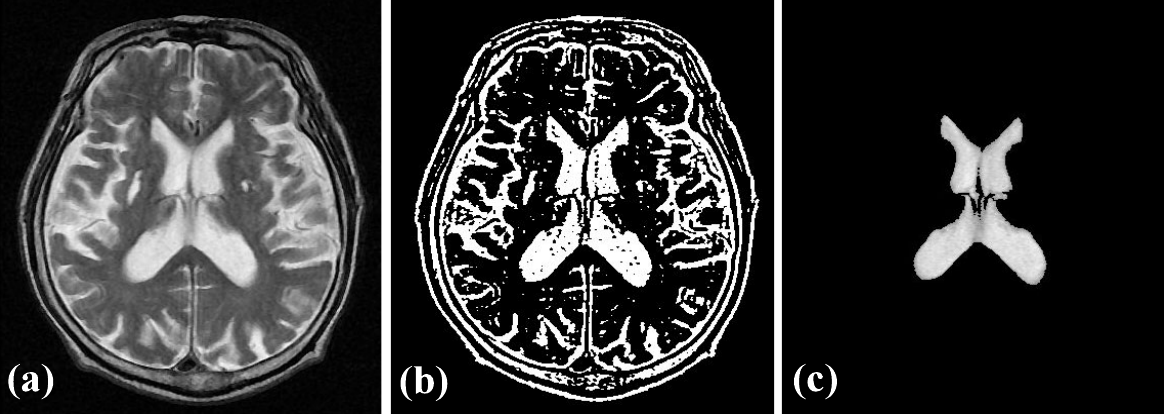
\includegraphics[width=\textwidth]{Images/4_extract_ventricle.png}
	\caption{Extraction of the cerebral ventricle.}
	\small Image taken from \cite{Yokoyama2007}
\end{figure}

Isolated lacune candidates were determined by extracting the cerebral ventricle and determining the mean pixel value of that region. The threshold for lacune identification was set at 70\% of the mean value. Yokoyama et al. claim that lacunes primarily occur in the basal ganglia, a structure at the centre of the brain. As a result, the detection region was limited to this area. Yokoyama et al. determined the coordinates bounding the cerebral centricle, which were then used to define a circular search region.

Lacunes were identified by considering three properties: area, circularity and gravitational centre.

\textit{Area}, $A$, is defined as the number of pixels that the candidate lacune covers. 

\textit{Circularity} is defined as
\[
	C = 4\pi \times \dfrac{A}{l^2},
\]
where $l$ is the perimeter of the candidate lacune.

The \textit{gravitational centre} is defined as the mean intensity of the pixels in the candidate lacune,
\[
	(g_x, g_y) = \bigg(\dfrac{1}{n}\sum_{i=1}^nx_i, \dfrac{1}{n}\sum_{i=1}^ny_i\bigg).
\]

% Fig. 5 from Yokoyama 2007 showing the bounds for area and circularity for false and true lacunes.

Candidate lacunes were then found to satisfy
\begin{align*}
	& 19 \le A \le 200, \\
	& 0.45 \le C,\text{ and } \\
	& (g_x - c_x)^2 + (g_y - c_y)^2 < 12000,
\end{align*}
where $(c_x, c_y)$ is the center of the circular region of interest.

For lacunes that appear next to white matter hyperintensities, the candidate region is more difficult to extract. To detect lacunes, Yokoyama et al. use the difference between two circular filters of radii 1 and 8 pixels. To eliminate false-positives, Yokoyama et al. considered a small change in pixel intensity between lacunar infarcts and cerebral ventricle CSF, using region growing techniques to detect circular features.

Using the same definitions for area and circularity as with isolated lacunes, candidates next to white matter hyperintensities satisfy
\[
	25 \le A \le 100\text{ and } 0.48 \le C.
\]

Once candidate lacunes have been identified, Yokoyama et al. then eliminated false positives by examining the T1-weighted scans. Removal of candidates is based on the location of the candidate, and on the area and gravitational centre as defined previously.

The algorithm was trained on 100 scans, containing 832 slices in total. 20 of these scans were used for training and 80 for testing. The algorithm achieved a testing sensitivity of 90.1\%, with an average of 1.7 false positives per slice.

The second phase of training reduced the number of false positives by 68\%. However, of the four types of false positives, enlarged perivascular spaces had no reduction. This model is instead more likely to differentiate lacunes from the edge of the cerebrum, hyperintensities and the cerebral ventricle.

Yokoyama et al. suggest that further reductions in false positives could be attained through the use of FLAIR imaging. Lacunes are found to have a low intensity in T1-weighted imaging and a high intensity in T2-weighted imaging. In FLAIR imaging, lacunes are also found to have a low intensity, but not as low as the surrounding CSF, and often have a hyperintense rim \cite{WardlawJ.M.2013Nsfr}. 

Further improvements could be made by using multiple slices for each candidate, increasing image context. Using 3D information, the axial slices above and below a candidate could be used to further eliminate false positives. This is particularly relevant when a candidate lacune appears on only a single axial slice, or when the candidate diverges from the usual ovoid shape in surrounding slices. Including this information would assist in differentiation between lacunes and perivascular spaces, since perivascular spaces can appear oblong along the coronial or saggital plane.

\subsection*{Concerns}

Although the testing sensitivity was high, it was not high enough for the model to be usable on its own. Model improvement is required before it can be used to aid clinicians reliably.

Yokoyama et al. made the assumption that lacunes only occur deep within the brain, within and surrounding the basal ganglia. This was the motivation behind extracting the cerebral ventricle. However, this assumption is not always satisfied. Though less common, lacunes have been found in other brain regions, including the cerebrum. As such, the analysis of only the deep central structures eliminates the possibility of identifying lacunes outside of that region.

The feature definitions used for the model also make it difficult to identify perivascular spaces. In this model, perivascular spaces were defined as small, circular regions of diameter less than 3mm, located at the lower basal ganglia. This specification meant that the model was not sensitive to enlarged perivascular spaces, which can have a diameter up to 10mm and can occur anywhere in the grey and white matter of the brain. This change in definition contributes to the seemingly low false positive presence that PVS exhibit in the data.

% Table 1 from Yokoyama 2007. Elimination of false positives - all PVS got through!
\begin{figure}[ht]
	\centering
	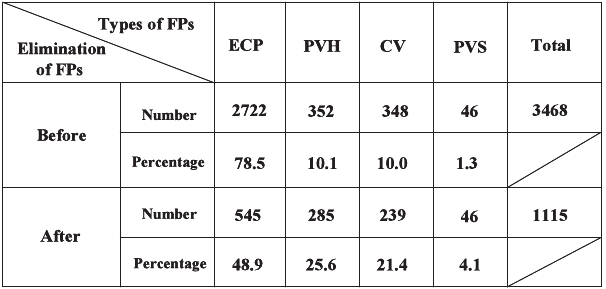
\includegraphics[width=0.8\textwidth]{Images/4_yokoyama2007testing.png}
	\caption{Elimination of false positives. Perivascular spaces (PVS) see no reduction. They make only 4.1\% of false positives under their definition.}
	\small Image taken from \cite{Yokoyama2007}
\end{figure}

It should be mentioned that this model is dependent on a number of existing architectures. The first is the identification and extraction of particular brain regions. In this model, Yokoyama et al. were able to use existing binarisation techniques to extract the cerebral ventricle. Each sample also requires a calculated area, circularity and gravitational centre. Each of these calculations requires sufficient time and resources, particularly if these calculations are to be conducted manually.

Finally, the proportion of false positives is still relatively high. The sensitivity after the second phase is 90\%, which is substantial but still not accurate enough to warrant full automation of the process. Of particular concern is the proportion of perivascular spaces falsely marked as lacunes. Though they appear similar to lacunes, perivascular spaces do present some slight shape and intensity differences.


\section{Support Vector Machines}

In 2007, Uchiyama et al. \cite{Uchiyama20071554} used a machine learning algorithm to develop a computer-assisted diagnosis (CAD) program for lacune identification. In particular, false positive reduction took the form of a support vector machine (SVM).

Their data consisted of 132 MRI scans, each with T1-weighted and T2-weighted images, giving a total of 1143 axial slices in the dataset. 

Similar to the method conducted by Yokoyama et al. \cite{Yokoyama2007}, Uchiyama et al. identified candidate lacunes of two forms: isolated lacunes, and those close to the cerebral ventricle. Isolated lacunes were determined by establishing a threshold, as these points exhibit a higher intensity compared to the surrounding tissue. For lacunes close to the cerebral ventricle, their higher intensity can be masked by the intensity of the surrounding ventricle. To address this, Uchiyama et al. used top-hat transforms on the T2-weighted images, a method that is specialised for extracting small details from image data.

% Candidate lacune identification
\begin{figure}[ht]
	\centering
	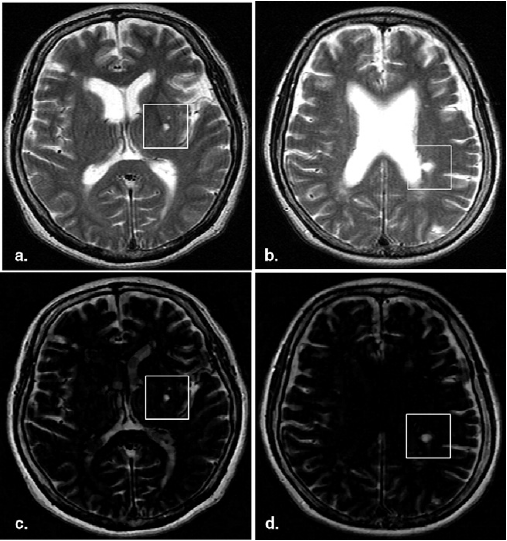
\includegraphics[width=0.8\textwidth]{Images/4_uchiyama_candidates.png}
	\caption{Candidate lacune detection. Isolated lacune in a), with resulting top-hat transform shown in c). Lacune in b) is next to the cerebral ventricle, with top-hat transform shown in d).}
	\small Image taken from \cite{Uchiyama20071554}
\end{figure}

False positives were reduced using support vector machines. 12 features were used in false positive reduction, including the candidate's x and y location, signal differences in the T1-weighted and T2-weighted images, and filtered images based on 4 nodular components and 4 combined nodular and linear components. This model produced a sensitivity of 96.8\%, with 0.76 false positives per slice.

\subsection*{Concerns}

Model sensitivity is high enough to warrant usage of the model, though not high enough for full dependency. As described by Uchiyama et al., the model was designed as a CAD scheme, to run alongside manual rating by clinicians. The model still requires a user to oversee and confirm its results. 
 
Similar to the model developed by Yokoyama et al. \cite{Yokoyama2007}, the model developed by Uchiyama et al. was not able to distinguish between lacunes and enlarged perivascular spaces. Despite the data containing analysis on the nodular and linear nature of the candidate, the model was unable to make this distinction. Therefore, users of the CAD system must take care to confirm that the suggested candidates are not enlarged perivascular spaces.

Many of the variables included in the method are dependent on other existing techniques. For instance, Uchiyama et al. explain that the nodular and linear components were determined via a newly explored filter bank technique. This technique was not well described, and as such, the model may be difficult to recreate.

Another issue is the coordinate system. The model uses the x and y coordinates of the candidate to reduce false positives. The coordinates themselves do not have any innate information about the structure of the brain. It is possible for the same x and y values to link to differing regions across brain scans. It is not certain that particular coordinates will align with a brain structure that has a significant influence on the presence of lacunes. This is especially the case for candidates deep in the brain, as many brain structures sit close together. 

Under the assumption that the x and y coordinates are indicative of lacune probability, the usage of location data may still incorrectly influence outcomes. Lacunes can be found throughout the brain, including in the cerebrum. 

\section{Neural Networks}

Uchiyama et al. \cite{Uchiyama2007b} improve their previous model \cite{Uchiyama20071554} by altering the method used for reducing false positives. The support vector machine was swapped with a neural network, using the same 12 input features.

The sensitivity of the model to lacunar infarcts remains the same, at 96.8\%. The number of false positives drops to 0.30 false positives per slice.

\section{Convolutional Neural Networks}
 
Ghafoorian et al. \cite{GhafoorianM.2017Dml3} utilised the fully convolutional nature of the initial detection model. This allows for fast image processing in comparison to fully connected layers, for 3D volumes. In addition, Ghafoorian et al. additionally utilised a multi-resolution convolutional neural network, along with 7 additional location features for false positive reduction.

\section{xgboost}

\section{Multi-Scale Location-Aware 3D CNN}\label{litrev-ghafoorian}

Entire model is made up of two neural networks.

The first is trained such that it detects candidate lacunes.

The second then takes the candidate lacunes, and processes them through a more thorough 3D CNN to finalise the outcome.

\subsection{First Phase - Candidate Detection}

Takes in 51x51 samples, where the T1 and FLAIR components are treated as separate channels. Twice as many negative samples as positive, with a total of 320K for training.

Seven layer CNN:
- 4 convolutional, with 20, 40, 80, 110 filters, with size 7x7, 5x5, 3x3, 3x3 respectively.
- 1 pooling layer: size 2x2, stride 2, after first conv layer
- 3 fully connected layers: sizes 300, 200 and 2
- Softmax output layer

All neurons went under batch normalisation.

Weights initialised by the He method.

ReLU activation to prevent vanishing gradient problem

Dropout of 0.3 on fully connected layers

Training conducted by stochastic gradient descent, Adam optimiser. Learning rate decayed, from 5e-4 to 1e-6

Batch size of 128

Categorical cross-entropy loss, with L2-regularisation (Ridge regression), lambda2 = 0.0001

Early stopping - model with highest accuracy on validation set


This method can be slow on its own. Translate the fully connected layers to convolutional layers, via shift-and-stitch method.

Local maxima extraction (10x10 window) - picking those with likelihood lower than 0.1.


Didn't mention: number of epochs to train. How pooling and convolutions were padded. Diagram implied no padding, but diagram dimensions weren't correct. 

\subsection{Second Phase - False Positive Reduction}

This model uses data at different scales around each candidate lacune. 

Input data of each point at three different scales: 32x32x5, 64x64x5, 128x128x5.

Each of these scales is reduced to 32x32x5, then put through a separate branch of the network.

385K training, 35K validation.

Three separate branches of convNets, one for each scale. Each branch contains:
 - 6 conv layers (64, 64, 128, 128, 256,256 filters, with sizes 3x3x2, 3x3x2, 3x3x1, 3x3x1, 3x3x1, 3x3x1)
 - 1 pooling, size 2x2x1, placed after second conv layer
 - Fully connected layer of 300 neurons
 
 The 3x300 fully connected neurons were concatenated with 7 addition location feature inputs.
 
 These location features include:
  - x,y,z coordinates
  - distances from left ventricle, right ventricle, cortex and midsaggital brain surface.

Then the 907 neurons are fully connected to two more fully connected layers, of size 200 and 2 neurons. 
These are fed through a softmax classifier to output the final result.

All weights are He initialised 

All activations are ReLU, and are batch normalised.

Fully connected layers have a dropout of 0.5.

Cost function is cross entropy with L2 regularisation, lambda2 = 2e-5. 

Stochastic gradient descent, Adam optimiser. Decaying learning rate, from 5e-4, decay factor of 2 when training accuracy dropped. 

Training for 40 epochs, batch size of 128.

Chose model with highest validation accuracy. 

Hyper-parameters were also chosen such as to attain highest validation accuracy. These hyper-parameters included network depth, batch size, initial learning rate, learning decay factor, lambda2 and dropout rate. This is done during the validation stage. Make several models, with differing hyper-parameters, with performance compared using the validation set. Then whichever model performs best on this validation set is chosen, and final performance judged by the test set.

Data was augmented during test time: cropping and flipping. Predictions of the 242 variants per sample were averaged.

Didn't mention: stride of pooling. Assumed 2 from diagram.
 
\subsection{Model performance}
 
%Famous Image Recognition Models
\section{ImageNet}


%%%%%%%%%%%%%%%%%%%%%%%%%%%%%%%%%%%%%%%%%%%%%%%%%%%%%%%%%%%%%%%%%%%%%%%%%%

\clearpage

\addcontentsline{toc}{chapter}{References}

\bibliographystyle{apalike}
\bibliography{bibliography.bib}

%\bibliographystyle{apacite}
%\bibliography{mybib.bib}

